\section{Daily PGP usage}

In the previous chapters we have have explained how to set up a secure
mail environment using Thunderbird, GPG and Enigmail. We assume you have
installed the software and have successfully followed the wizard
instructions to generate an encryption key-pair as described in the
previous chapter. This chapter will describe how to use your secured
Thunderbird in daily life to protect your e-mail communication. In
particular we will focus on:

\begin{enumerate}[1.]
\item
  Encrypting attachments
\item
  Entering your pass-phrase
\item
  Receiving encrypted e-mail
\item
  Sending and receiving public keys
\item
  Receiving public keys and adding them to your key ring
\item
  Using public key servers
\item
  Signing e-mails to an individual
\item
  Sending encrypted e-mails to an individual
\item
  Automating encryption to certain recipients
\item
  Verifying incoming e-mails
\item
  Revoking your GPG key pair
\item
  What to do when you have lost your secret key, or forgot your
  passphrase
\item
  What to do when your secret key has been stolen, or compromised
\item
  Backing up your keys
\end{enumerate}
First we shall explain two dialog windows that will inevitably appear
after you start using Thunderbird to encrypt your emails.

\subsection{Encrypting attachments}

The dialog window below will pop-up whenever you are sending an
encrypted email with attachments for the first time. Thunderbird asks a
technical question on how to encrypt attachments to your mail. The
second (default) option is the best choice, because it combines security
with the highest compatibility. You should also select the `Use the
selected method for all future attachments' option. Then click `OK' and
your mail should be sent with no further delay.

\begin{figure}[htbp]
\centering
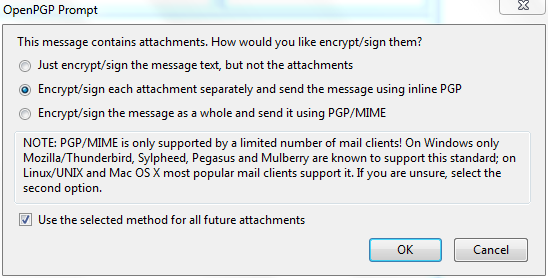
\includegraphics{daily_gpg_1.png}
\caption{Daily GPG Usage}
\end{figure}

\subsection{Entering your pass-phrase}

For security reasons, the pass-phrase to your secret key is stored
temporarily in memory. Every now and then the dialog window below will
pop-up. Thunderbird asks you for the pass-phrase to your secret key.
This should be different from your normal email password. It was the
pass-phrase you have entered when creating your key-pair in the previous
chapter. Enter the pass-phrase in the text-box and click on `OK'

\begin{figure}[htbp]
\centering
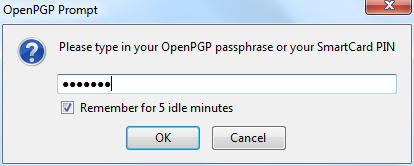
\includegraphics{daily_gpg_2.png}
\caption{Daily GPG Usage}
\end{figure}

\subsection{Receiving encrypted e-mails}

The decryption of e-mails is handled automatically by Enigmail, the only
action that may be needed on your behalf is to enter the pass-phrase to
your secret key. However, in order to have any kind of encrypted
correspondence with somebody, you will first need to exchange public
keys.

\subsection{Sending and receiving public keys}

There are multiple ways to distribute your public key to friends or
colleagues. By far the simplest way is to attach the key to a mail. In
order for your friend to be able to trust that the message actually came
from you, you should inform them in person (if possible) and also
require them to reply to your mail. This should at least prevent easy
forgeries. You have to decide for yourself what level of validation is
necessary. This is also true when receiving emails from third-parties
containing public keys. Contact your correspondent through some means of
communication other than e-mail. You can use a telephone, text messages,
Voice over Internet Protocol (VoIP) or any other method, but you must be
absolutely certain that you are really talking to the right person. As a
result, telephone conversations and face-to-face meetings work best, if
they are convenient and if they can be arranged safely.

Sending your public key is easy.

\begin{enumerate}[1.]
\item
  In Thunderbird, click on the 
\includegraphics{gpg_write.png} icon.
\item
  Compose a mail to your friend or colleague and tell them you are
  sending them your PGP public key. If your friend does not know what
  that means, you may have to explain them and point them to this
  documentation.
\item
  Before actually sending the mail, click to
  \verb!OpenPGP > Attach My Public Key! option on the menu bar of the
  mail compose window. Next to this option a marked sign will appear.
  See the example below.
\end{enumerate}
\begin{figure}[htbp]
\centering
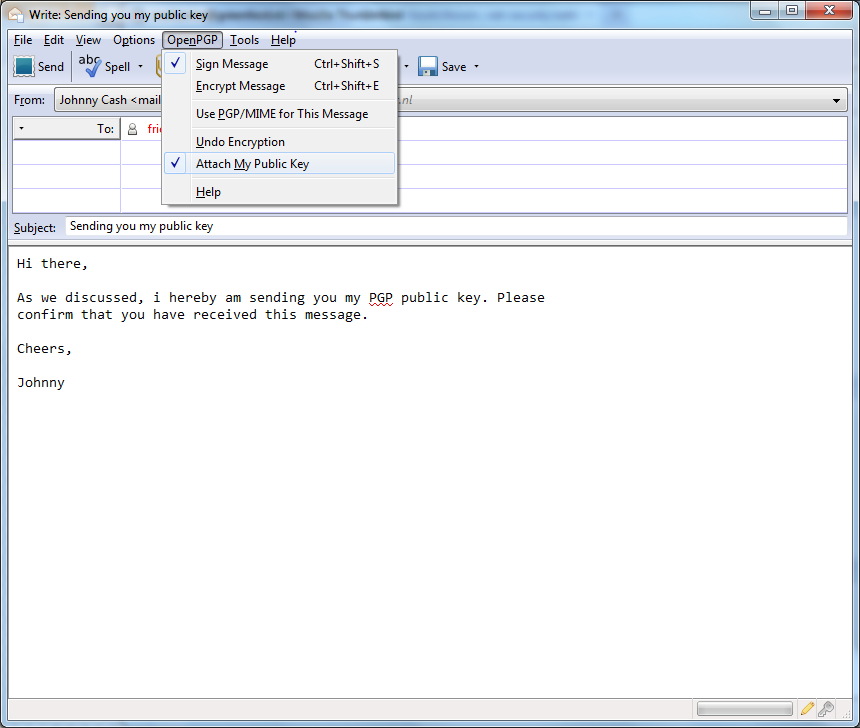
\includegraphics{daily_gpg_3.png}
\caption{Daily GPG Usage}
\end{figure}

\begin{enumerate}[1.]
\setcounter{enumi}{3}
\item
  Send your mail by clicking on the 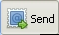
\includegraphics{gpg_send.png}
  button.
\end{enumerate}
\subsection{Receiving public keys and adding them to your keyring}

Lets say we receive a public key from a friend by mail. The key will
show up in Thunderbird as an \emph{attached file}. Scroll down the
message and below you will find tabs with one or two file names. The
extension of this public key file will be .asc, different from the
extension of an attached GPG signature, which ends with .asc.sig

Look at the example email in the next image, which is a received, signed
GPG message containing an attached public key. We notice a yellow bar
with a warning message: `OpenPGP: Unverified signature, click on
'Details' button for more information'. Thunderbird warns us that the
sender is not known yet, which is correct. This will change once we have
accepted the public key.

What are all those strange characters doing in the mail message? Because
Thunderbird does not yet recognize the signature as valid, it prints out
the entire raw signature, just as it has received it. This is how
digitally signed GPG messages will appear to those recipients who do not
have your public key.

The most important thing in this example is to find the attached GPG
public key. We mentioned it is a file that ends with .asc. In this
example it's the first attachment on the left, in the red circle.
Double-clicking on this attachment will make Thunderbird recognize the
key.

\begin{figure}[htbp]
\centering
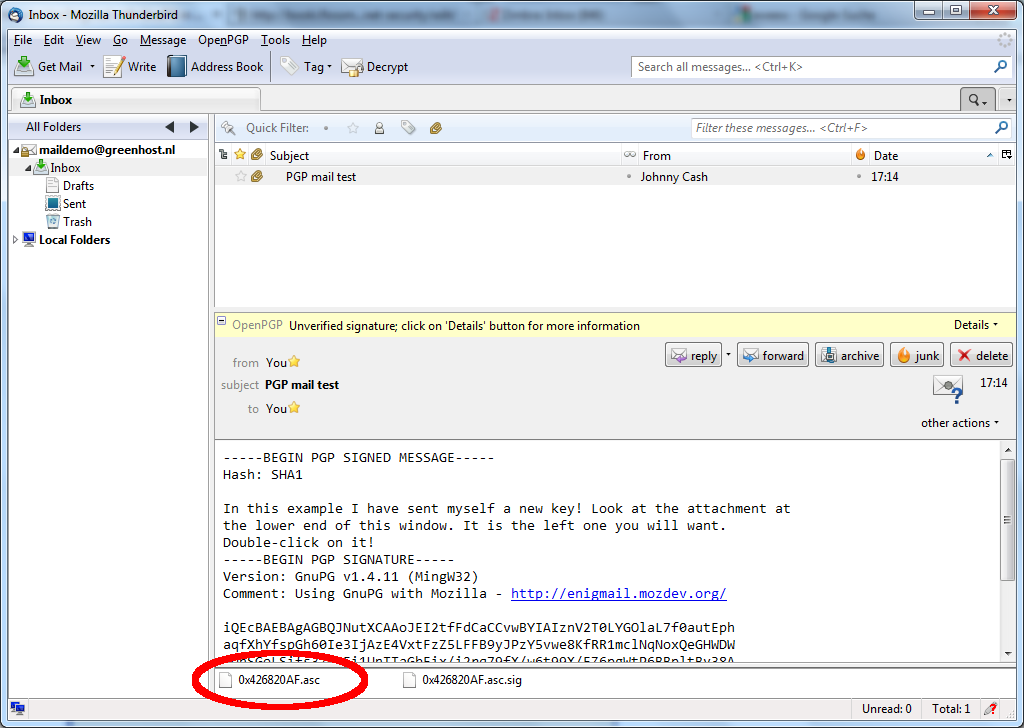
\includegraphics{daily_gpg_4.png}
\caption{Daily GPG Usage}
\end{figure}

After we have clicked on the attachment, the following pop-up will
appear.

\begin{figure}[htbp]
\centering
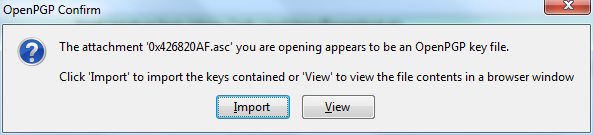
\includegraphics{daily_gpg_5.png}
\caption{Daily GPG Usage}
\end{figure}

Thunderbird has recognized the GPG public key file. Click on `Import' to
add this key to your keyring. The following pop-up should appear.
Thunderbird says the operation was successful. Click on `OK' and you are
almost done.

\begin{figure}[htbp]
\centering
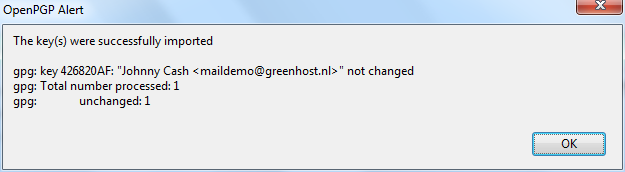
\includegraphics{daily_gpg_6.png}
\caption{Daily GPG Usage}
\end{figure}

We are back in the main Thunderbird screen and we refresh the view on
this particular example message, by clicking on some other message and
back for example. Now the body of the message looks different (see
below). This time Thunderbird \emph{does} recognize the signature,
because we have added the public key of the sender.

\begin{figure}[htbp]
\centering
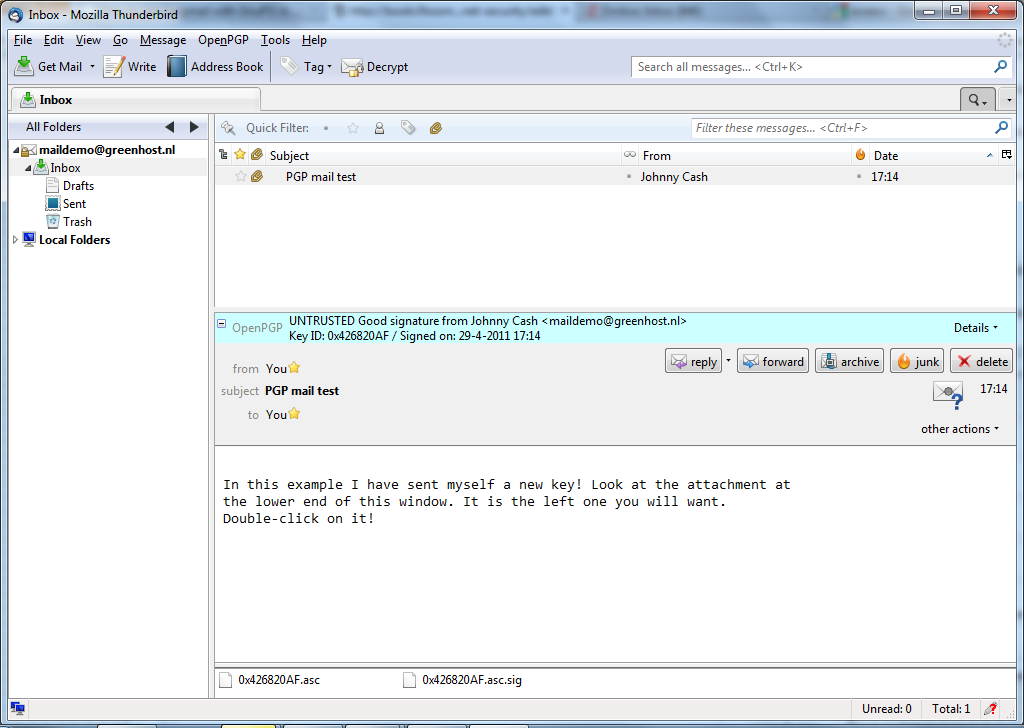
\includegraphics{daily_gpg_7.png}
\caption{Daily GPG Usage}
\end{figure}

There is still one thing that remains. While Thunderbird now recognizes
the signature, we should explicitly trust that the public key really
belongs to the sender in real life. We realize this when we take a
closer look at the green bar (see below). While the signature is good,
it is still UNTRUSTED.

\begin{figure}[htbp]
\centering

\includegraphics{daily_gpg_8.png}
\caption{Daily GPG Usage}
\end{figure}

We will now decide to trust this particular public key and the
signatures made by it. We can do this immediately by clicking on
`Details'. A small menu will appear (see below). From this menu we
should click on the option `Sign Sender's Key \ldots{}'.

\begin{figure}[htbp]
\centering
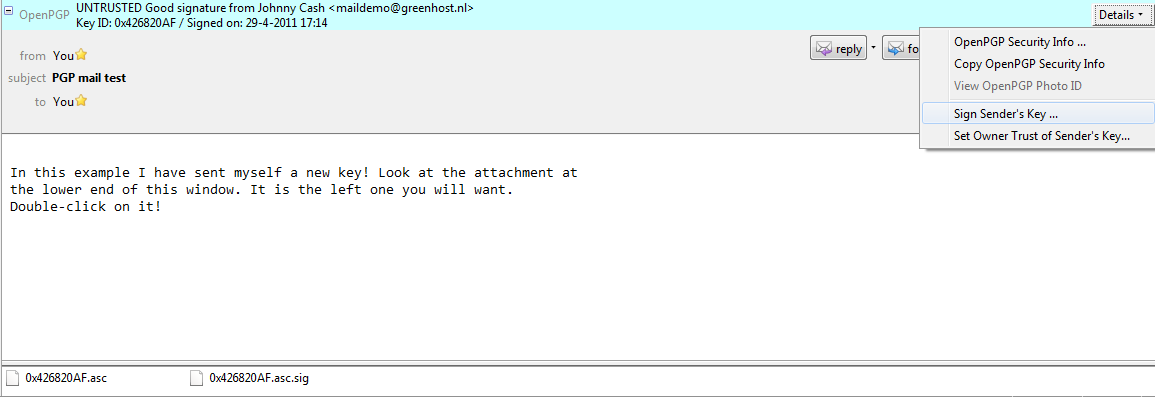
\includegraphics{daily_gpg_9.png}
\caption{Daily GPG Usage}
\end{figure}

After we have selected `Sign Sender's Key \ldots{}' we will get another
selection window (see below). We are requested to state how carefully we
have checked this key for validity. The explanation of levels of trust
and trust networks in GPG falls outside the scope of this document. We
will not use this information, therefore we will just select the option
`I will not answer'. Also select the option `Local signature (cannot be
exported)'. Click on the `OK' button to finishing signing this key. This
finishes accepting the public key. You can now send encrypted mail to
this individual.

\begin{figure}[htbp]
\centering
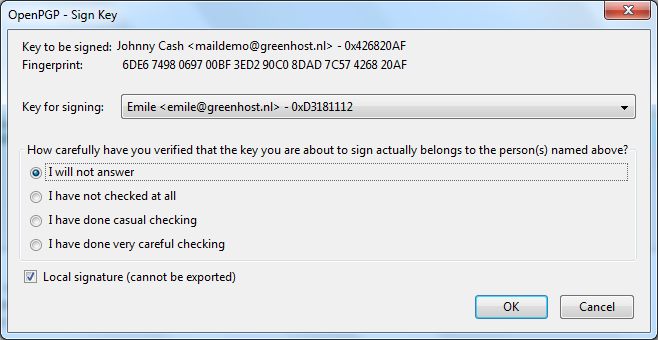
\includegraphics{daily_gpg_10.png}
\caption{Daily GPG Usage}
\end{figure}

\subsection{Using public key servers}

Another method of distributing public keys is by putting them on a
public key server. This allows anyone to check whether your email
address has GPG support, and then download your public key.

To put your own key on a keyserver, take the following steps.

\begin{enumerate}[1.]
\item
  Head to the key manager by using the Thunderbird menu and click on
  \verb!OpenPGP > Key Management!
\end{enumerate}
\begin{figure}[htbp]
\centering
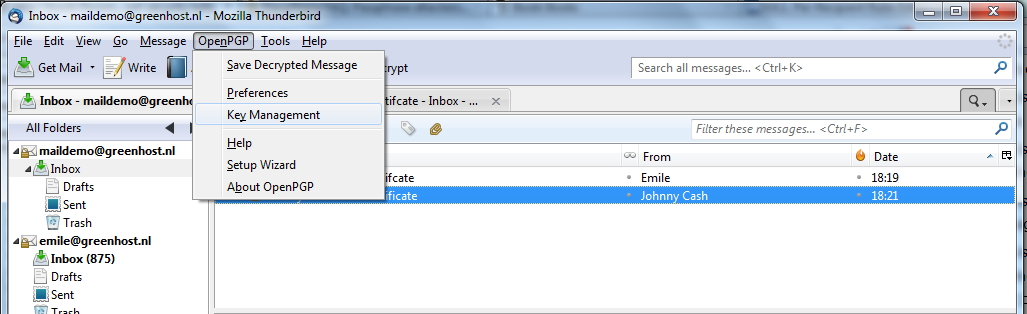
\includegraphics{daily_gpg_11.png}
\caption{Daily GPG Usage}
\end{figure}

\begin{enumerate}[1.]
\setcounter{enumi}{1}
\item
  The key management window will be displayed and looks like this:
\end{enumerate}
\begin{figure}[htbp]
\centering
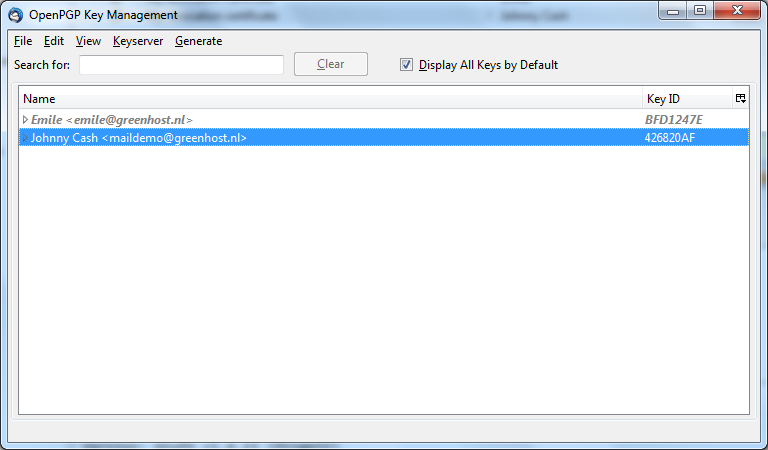
\includegraphics{daily_gpg_12.png}
\caption{Daily GPG Usage}
\end{figure}

\begin{enumerate}[1.]
\setcounter{enumi}{2}
\item
  You need to have selected the `Display All Keys by Default' option to
  get a list of all your keys. Look up your own email address in the
  list and right click on the address. A selection window will appear
  with some options. Select the option `Upload Public Keys to
  Keyserver'.
\end{enumerate}
\begin{figure}[htbp]
\centering
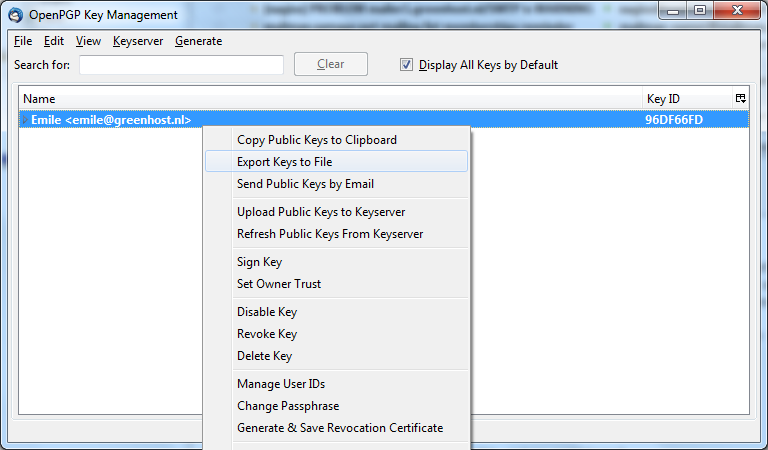
\includegraphics{daily_gpg_13.png}
\caption{Daily GPG Usage}
\end{figure}

\begin{enumerate}[1.]
\setcounter{enumi}{3}
\item
  You will see a small dialog window like below. The default server to
  distribute your keys to is good. Press 'OK" and distribute your public
  key to the world.
\end{enumerate}
\begin{figure}[htbp]
\centering
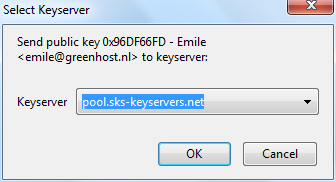
\includegraphics{daily_gpg_14.png}
\caption{Daily GPG Usage}
\end{figure}

To look up whether some email address has a public key available on a
server, take the following steps.

\begin{enumerate}[1.]
\item
  Head to the key manager by using the Thunderbird menu and click on
  \verb!OpenPGP > Key Management!
\item
  In the key manager window menu bar, select
  \verb!Keyserver > Search for Keys!
\end{enumerate}
\begin{figure}[htbp]
\centering
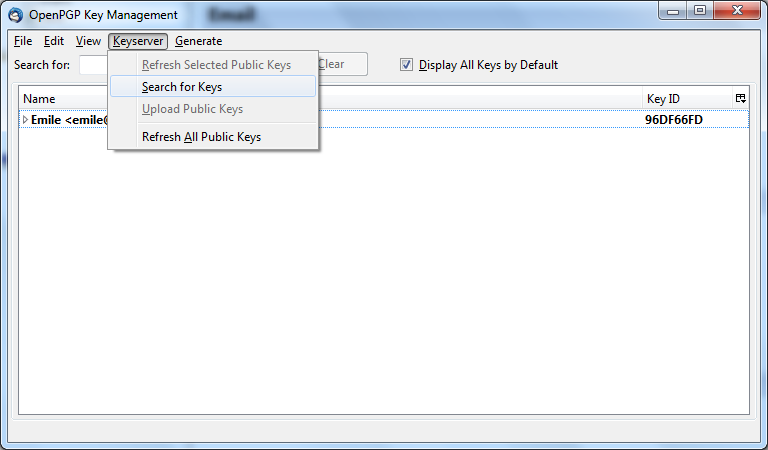
\includegraphics{daily_gpg_15.png}
\caption{Daily GPG Usage}
\end{figure}

\begin{enumerate}[1.]
\setcounter{enumi}{2}
\item
  In this example we will look-up up the key for the creator of PGP
  software, Philip Zimmermann. After we have entered the email address,
  we click on `OK'.
\end{enumerate}
\begin{figure}[htbp]
\centering
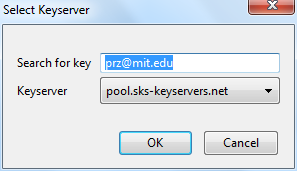
\includegraphics{daily_gpg_16.png}
\caption{Daily GPG Usage}
\end{figure}

\begin{enumerate}[1.]
\setcounter{enumi}{3}
\item
  The next window displays the result of our search. We have found the
  public key. It is automatically selected. Just click on `OK' to import
  the key.
\end{enumerate}
\begin{figure}[htbp]
\centering
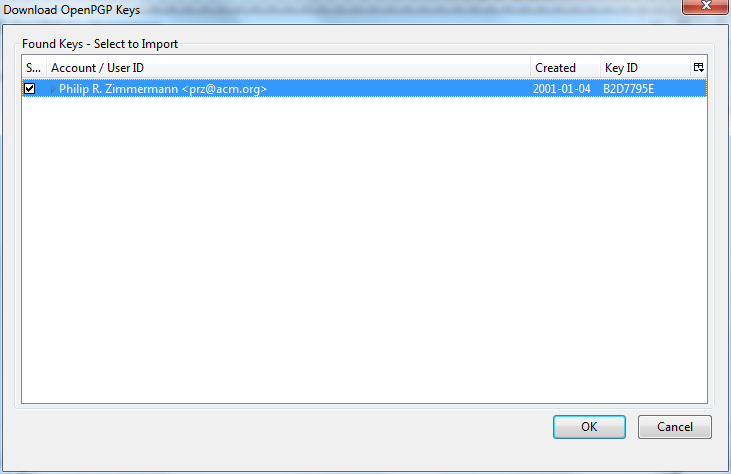
\includegraphics{daily_gpg_17.png}
\caption{Daily GPG Usage}
\end{figure}

\begin{enumerate}[1.]
\setcounter{enumi}{4}
\item
  Importing the key will take some time. On completion you should see a
  pop-up window like below.
\end{enumerate}
\begin{figure}[htbp]
\centering
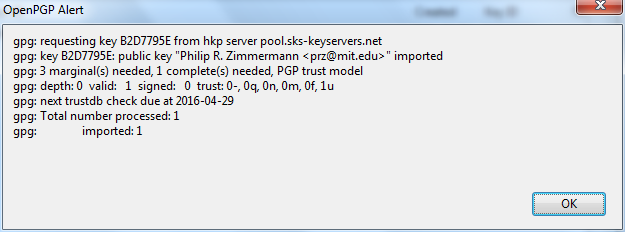
\includegraphics{daily_gpg_18.png}
\caption{Daily GPG Usage}
\end{figure}

\begin{enumerate}[1.]
\setcounter{enumi}{5}
\item
  The final step is to locally sign this key, to indicate that we trust
  it. When you are back in the key manager, make sure you have selected
  the `Display All Keys by Default' option. You should now see the newly
  imported key in the list. Right-click on the address and select the
  option `Sign Key' from the list.
\end{enumerate}
\begin{figure}[htbp]
\centering
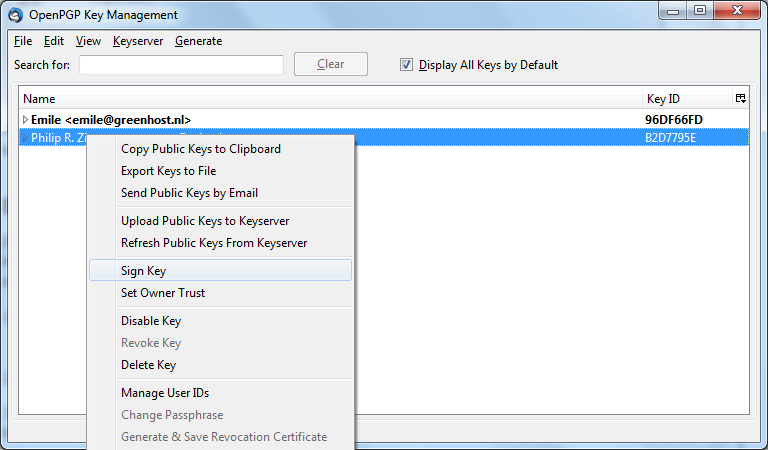
\includegraphics{daily_gpg_19.png}
\caption{Daily GPG Usage}
\end{figure}

\begin{enumerate}[1.]
\setcounter{enumi}{6}
\item
  Select the options `I will not answer' and `Local signature (cannot be
  exported)', then click on `OK'. You are now finished and can send
  Philip Zimmermann encrypted mail.
\end{enumerate}
\begin{figure}[htbp]
\centering
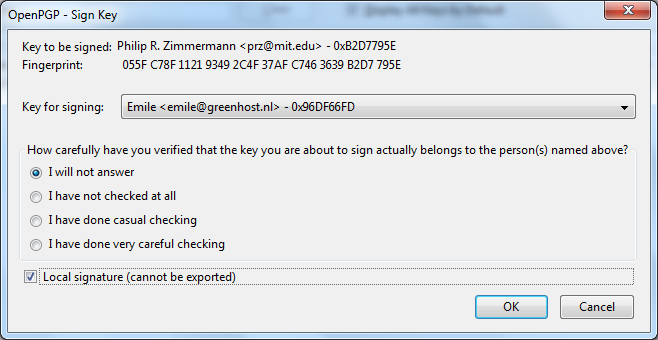
\includegraphics{daily_gpg_20.png}
\caption{Daily GPG Usage}
\end{figure}

\subsection{Signing emails to an individual}

Digitally signing email messages is a way to prove to recipients that
you are the actual sender of a mail message. Those recipients who have
received your public key will be able to \emph{verify} that your message
is authentic.

\begin{enumerate}[1.]
\item
  Offer your friend your public key, using the method described earlier
  in this chapter.
\item
  In Thunderbird, click on the 
\includegraphics{gpg_write.png} icon.
\item
  Before actually sending the mail, enable the
  \verb!OpenPGP > Sign Message! option via the menu bar of the mail
  compose window, if it is not enable already. Once you have enabled
  this option, by clicking on it, a marked sign will appear. Clicking
  again should disable encryption again. See the example below.
\end{enumerate}
\begin{figure}[htbp]
\centering
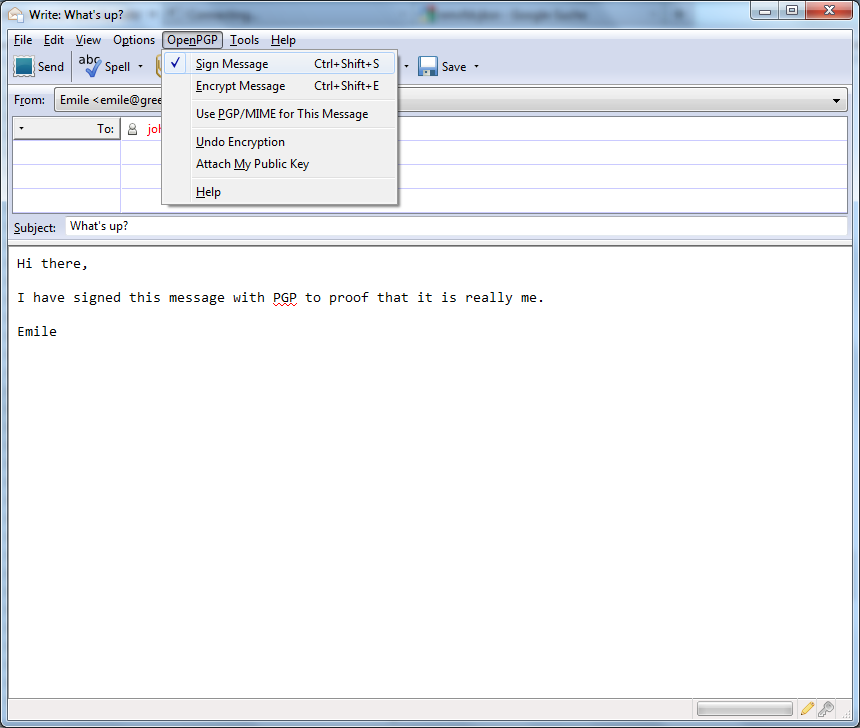
\includegraphics{daily_gpg_21.png}
\caption{Daily GPG Usage}
\end{figure}

\begin{enumerate}[1.]
\setcounter{enumi}{3}
\item
  Click on the 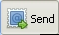
\includegraphics{gpg_send.png} button and your signed
  mail will be sent.
\end{enumerate}
\subsection{Sending encrypted mails to an individual}

\begin{enumerate}[1.]
\item
  You should have received the public key from the friend or colleague
  you want to email and you should have accepted their public key, using
  the method describe earlier in this chapter.
\item
  In Thunderbird, click on the 
\includegraphics{gpg_write.png} icon.
\item
  Compose a mail to the friend or colleague, from who you have
  previously received their public key. \textbf{Remember the subject
  line of the message will not be encrypted}, only the message body
  itself, and any attachments.
\item
  Before actually sending the mail, enable the
  \verb!OpenPGP > Encrypt Message! option via the menu bar of the mail
  compose window, if it is not enabled already. Once you have enabled
  this option, by clicking on it, a marked sign will appear. Clicking
  again should disable encryption again. See the example below.
\end{enumerate}
\begin{figure}[htbp]
\centering
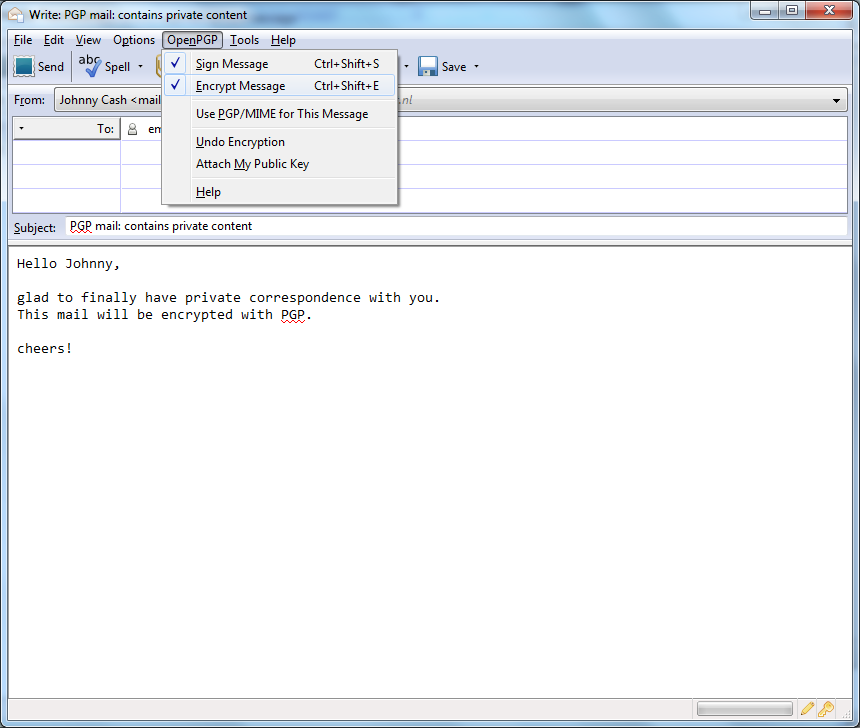
\includegraphics{daily_gpg_22.png}
\caption{Daily GPG Usage}
\end{figure}

\begin{enumerate}[1.]
\setcounter{enumi}{4}
\item
  Click on the 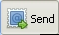
\includegraphics{gpg_send.png} button and your encrypted
  mail will be sent.
\end{enumerate}
\subsection{Automating encryption to certain recipients}

You will often want to make sure all your messages to a certain
colleague or friend are signed and encrypted. This is good practice,
because you may forget to enable the encryption manually. You can do
this by editing the per-recipient rules. To do this we access the
OpenPGP per-recipient rule editor.

Select \verb!OpenPGP > Preferences! from the Thunderbird menu bar.

\begin{figure}[htbp]
\centering
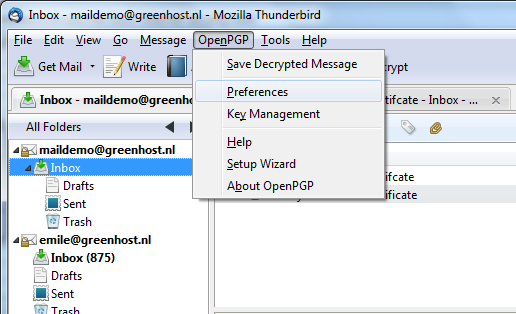
\includegraphics{daily_gpg_23.png}
\caption{Daily GPG Usage}
\end{figure}

The preferences window will appear like below. We need to click on
`Display Expert Settings'.

\begin{figure}[htbp]
\centering
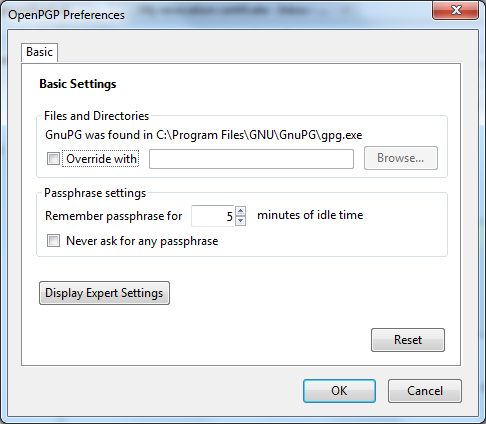
\includegraphics{daily_gpg_24.png}
\caption{Daily GPG Usage}
\end{figure}

New menu tabs will appear in the window. Go to the tab `Key Selection'
and then click on the button labeled `Edit Rules \ldots{}'

\begin{figure}[htbp]
\centering
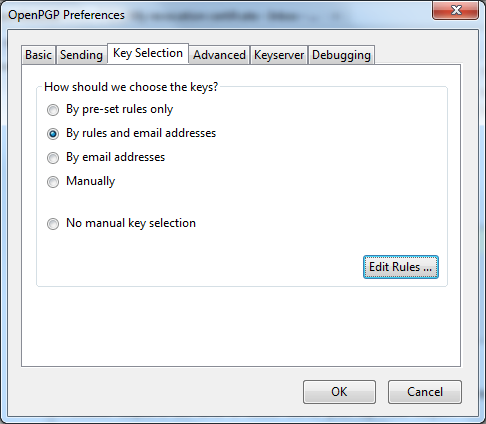
\includegraphics{daily_gpg_25.png}
\caption{Daily GPG Usage}
\end{figure}

We are now shown the per-recipient rules editor (see below). This editor
can be used to specify the way how messages to certain recipients are
sent. We will now add a rule saying we want to encrypt and sign all mail
messages to \verb!maildemo@greenhost.nl!

First click on the `Add' button.

\begin{figure}[htbp]
\centering
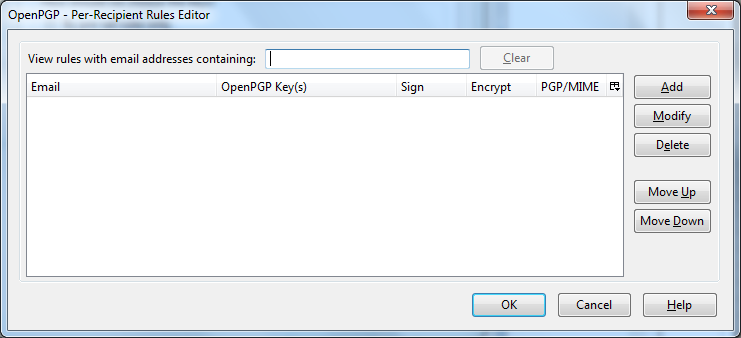
\includegraphics{daily_gpg_26.png}
\caption{Daily GPG Usage}
\end{figure}

Now the window to add a new rule will be shown.

The first thing we should enter is the email address of the recipient.
In the example below we have entered \verb!maildemo@greenhost.nl!

\begin{figure}[htbp]
\centering
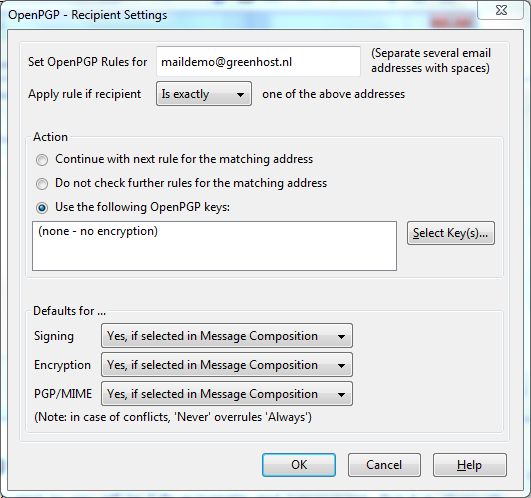
\includegraphics{daily_gpg_27.png}
\caption{Daily GPG Usage}
\end{figure}

Now we will set the encryption defaults by using the drop-downs below.
For Signing select `Always'. For Encryption also select `Always'.

\begin{figure}[htbp]
\centering
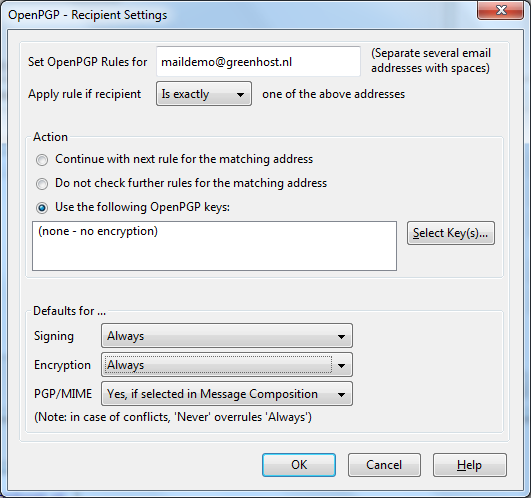
\includegraphics{daily_gpg_28.png}
\caption{Daily GPG Usage}
\end{figure}

Finally we have to select the \emph{public key} of the recipient, with
which to encrypt our messages. Do not forget this important step,
otherwise the e-mail will not be encrypted. Click on the button labeled
`Select Key(s)\ldots{}'. The key selection window will show up. The most
obvious key will be selected by default. In the example below, we only
have one public key available. We can select keys by clicking on the
small box next to the address. Then we click `OK' and close all relevant
windows and we are finished.

\begin{figure}[htbp]
\centering
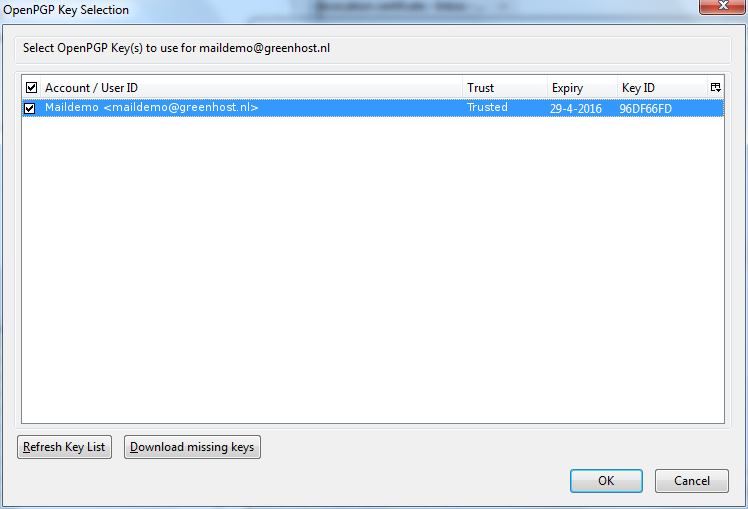
\includegraphics{daily_gpg_29.png}
\caption{Daily GPG Usage}
\end{figure}

\subsection{Verifying incoming e-mails}

Decrypting email messages sent to you will be fully automatic and
transparent. But it is obviously important to see whether or not a
message to you has in fact been encrypted or signed. This information is
available by looking at the special bar above the message body.

A valid signature will be recognized by a green bar above the mail
message like the example image below.

\begin{figure}[htbp]
\centering
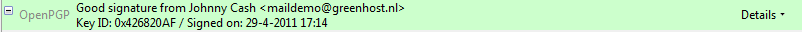
\includegraphics{daily_gpg_30.png}
\caption{Daily GPG Usage}
\end{figure}

The last example message was signed but not encrypted. If the message
had been encrypted, it would show like this:

\begin{figure}[htbp]
\centering
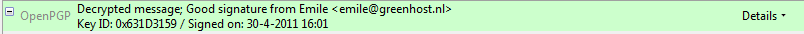
\includegraphics{daily_gpg_31.png}
\caption{Daily GPG Usage}
\end{figure}

When a message which has been encrypted, but not signed, it could have
been a forgery by someone. The status bar will become gray like in the
image below and tells you that while the message was sent securely
(encrypted), the sender could have been someone else than the person
behind the email address you will see in the `From' header. The
signature is neccessaty to verify the real sender of the message. Of
course it is perfectly possible that you have published your public key
on the Internet and you allow people to send you emails anonymously. But
is it also possible that someone is trying to impersonate one of your
friends.

\begin{figure}[htbp]
\centering

\includegraphics{daily_gpg_32.png}
\caption{Daily GPG Usage}
\end{figure}

Similarly if you receive a signed email from somebody you know, and you
have this persons public key, but still the status bar becomes yellow
and displays a warning message, it is likely that someone is attempting
to send you forged emails!

\begin{figure}[htbp]
\centering
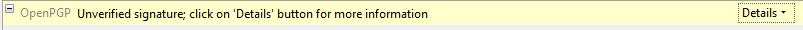
\includegraphics{daily_gpg_33.png}
\caption{Daily GPG Usage}
\end{figure}

Sometimes secret keys get stolen or lost. The owner of the key will
inform his friends and send them a so-called revocation certificate
(more explanation of this in the next paragraph). Revocation means that
we no longer trust the old key. The thief may afterwards still try his
luck and send you a falsely signed mail message. The status bar will now
look like this:

\begin{figure}[htbp]
\centering

\includegraphics{daily_gpg_34.png}
\caption{Daily GPG Usage}
\end{figure}

Strangely enough Thunderbird in this situation will still display a
green status bar! It is important to look at the contents of the status
bar in order to understand the encryption aspects of a message. GPG
allows for strong security and privacy, but only if you are familiar
with its use and concepts. Pay attention to warnings in the status bar.

\subsection{Revoking your GPG key-pair}

Your secret key has been stolen by somebody. Your harddisk crashed and
you have lost all your data. If your key is lost, you can no longer
decrypt messages. If your key has been stolen, somebody else can decrypt
your communication. You need to make a new set of keys. The process of
creating keys, using the OpenPGP wizard in Thunderbird, has been
described in this manual. But first you want to tell the world that your
old public key is now worthless, or even dangerous to use.

\subsection{What to do when you have lost your secret key, or forgot
your passphrase}

During the creation of your key-pair, the OpenPGP wizard offered you the
possibility to create a so-called revocation certificate. This is a
special file you send to others in the advent you have to disable your
key. If you have a copy of this file, sending the revocation key is
simply sending the file as an attachment to all your friends. You can no
longer send signed mails (obviously, because you have lost your secret
key). That doesn't matter. Send it as a normal mail. The revocation
certificate file could only have been created by the owner of the secret
key and proofs he or she wants to revoke it. That's why it should
normally be kept hidden from others.

If you do not have the revocation certificate, there exists no other
option than for you to contact your friends personally and convince them
your key is lost and that they should no longer trust it.

\subsection{What to do when your secret key has been stolen, or
compromised}

If you have reason to believe your secret key has been compromised, or
worse your secret key and passphrase, it is very important to contact
others that they should stop sending you encrypted messages. With your
secret key, other persons will be able to break the encryption of your
e-mail messages if they also have your passphrase. This is also true for
those messages you have send in the past. Cracking the passphrase is not
trivial, but it may be possible if the party has lots of resources, like
a state or a big organization for example, or if your passphrase is too
weak. In any case you should assume the worst and assume your passphrase
may have been compromised. Send a revocation certificate file to all
your friends or contact them personally and inform them of the
situation.

Even after you have revoked your old key pair, the stolen key may still
be used to decrypt your previous correspondence. You should consider
other ways to protect that old correspondence, for instance by
re-encrypting it with a new key. The latter operation will not be
discussed in this manual. If you are uncertain you should seek
assistance from experts or look up more information on the web.

\subsection{Receiving a revocation certificate}

If one of your friends sends you a revocation certificate, s/he asks you
to distrust his public key from now on. You should always accept such a
request and `import' the certificate to disable their key. The process
of accepting a revocation certificate is exactly the same as accepting a
public key, as has already been described in the chapter. Thunderbird
will ask you if you want to import the `OpenPGP key file'. Once you have
done so, a confirmation pop-up should be displayed like below.

\begin{figure}[htbp]
\centering
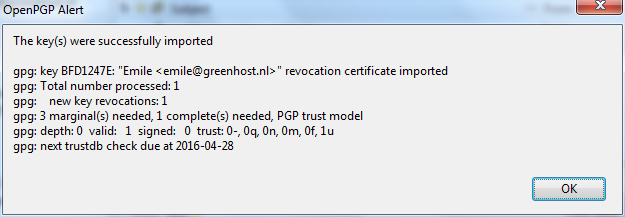
\includegraphics{daily_gpg_35.png}
\caption{Daily GPG Usage}
\end{figure}

\subsection{Preparing for the worst: backup your keys}

Your keys are usually stored on your hard disk as normal files. They may
get lost if your computer gets damaged. It is strongly advised to keep a
backup of your keys in a safe place, like a vault. Making a a backup of
your secret key has another security advantage as well. Whenever you
fear your laptop or computer is in immediate danger of being
confiscated, you can safely delete your key-pair. Your email will be
rendered unreadable immediately. At a later stage, you can retrieve your
keys from the vault and re-import them in Thunderbird.

To make a backup of your key-pair, first head to the key manager by
using the Thunderbird menu and click on \verb!OpenPGP > Key Management!.

You need to have selected the `Display All Keys by Default' option to
get a list of all your keys. Lookup your own email address in the list
and right click on the address. A selection window will appear with some
options. Select the option `Export Keys to File'.

\begin{figure}[htbp]
\centering
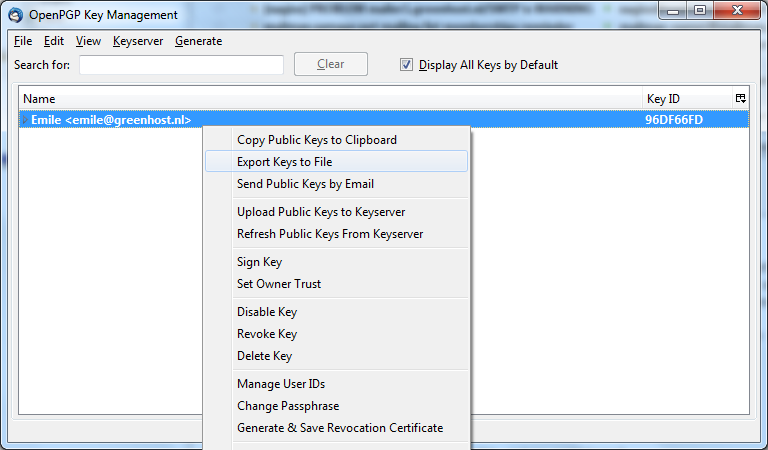
\includegraphics{daily_gpg_36.png}
\caption{Daily GPG Usage}
\end{figure}

Now we will save the key-pair to a file. Thunderbird asks us if we want
to include the secret key as well. We do want to include the secret key,
therefore we select `Export Secret Keys'.

\begin{figure}[htbp]
\centering
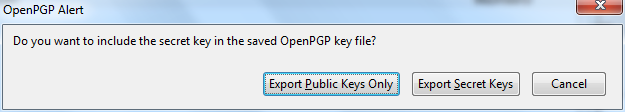
\includegraphics{daily_gpg_37.png}
\caption{Daily GPG Usage}
\end{figure}

Finally Thunderbird asks us for the location of the key file. You can
store the file anywhere you like, network disk, USB-stick. Just remember
to hide it away from other people.

\subsection{Further reading}

More documentation on using GPG with Thunderbird can be found on the
website of the Enigmail plugin. The Enigmail handbook is the guide you
will want to use.

\href{http://enigmail.mozdev.org/documentation/handbook.php.html}{http://enigmail.mozdev.org/documentation/handbook.php.html}
